\chapter{User documentation}
\label{ch:user}

Both the changes in the Clang-Tidy infrastructure and our new checker obviously focuses heavily on LLVM's Clang-Tidy.
Clang-Tidy is a clang-based C++ “linter” tool. Its purpose is to provide an extensible framework for diagnosing and fixing
typical programming errors, like style violations, interface misuse, or bugs that can be deduced via static analysis.
Clang-Tidy is modular and provides a convenient interface for writing new checks. % https://clang.llvm.org/extra/clang-tidy/

This tool can be found in the LLVM project repository. % https://github.com/llvm/llvm-project

\section{Install guide}

\subsection{System Requirements}

Table 2.1 shows the system requirements and supported compilers for building
LLVM. The checkers were developed with Ubuntu 20.04 and tested on Ubuntu 18.04, and WSL Ubuntu 20.04.

Building and using LLVM's Clang-Tidy takes a lot of time on weaker computers. The minimum recommended memory size
for building is 16 GB, the optimal amount is 64 GB of memory. % continue with the recommendation  

\begin{table}[H]
	\centering
	\begin{tabular}{ | m{0.33\textwidth} | m{0.33\textwidth} | m{0.33\textwidth} | }
		\hline
		\textbf{Operating System} & \textbf{Processor Architecture} & \textbf{Compiler} \\
		\hline \hline
		Linux & x861 & gcc, clang \\
		\hline
		Linux & amd64 & gcc, clang \\
		\hline
		Linux & arm & gcc, clang \\
		\hline
		Linux & Mips & gcc, clang \\
		\hline
		Linux & PowerPC & gcc, clang \\
		\hline
		Solaris & V9 & gcc \\
		\hline
		FreeBSD & x861 & gcc, clang \\
		\hline
		FreeBSD & amd64 & gcc, clang \\
		\hline
		NetBSD & x861 & gcc, clang \\
		\hline
		NetBSD & amd64 & gcc, clang \\
		\hline
		macOS2 & PowerPC & gcc \\
		\hline
		macOS & x86 & gcc, clang \\
		\hline
		Cygwin & x86 & gcc \\
		\hline
		Windows & x86 & Visual Studio \\
		\hline
		Windows64 & x86-64 & Visual Studio \\
		\hline
	\end{tabular}
	\caption{System requirements and supported compilers for building LLVM}
	\label{tab:example-1}
\end{table}

Software requirements include (at least) GCC version 7.1.0, CMake version 3.13.4, Python version 3.6 and GNU Make version 3.79.
% TODO cite? https://llvm.org/docs/GettingStarted.html#requirements

\subsection{Building from source}

These commands will compile LLVM from source. The building process with parameters can be found on the README.md of
LLVM project Github repository\footnote{https://github.com/llvm/llvm-project\#readme}, or the Getting
Started\footnote{https://clang.llvm.org/get_started.html} page of Clang documentation. These are the commands I used for
the compilation.
% https://github.com/llvm/llvm-project#readme and https://clang.llvm.org/get_started.html

\begin{lstlisting}[language={bash}]
	# On windows, git clone --config core.autocrlf=false https://github.com/llvm/llvm-project.git
	git clone https://github.com/llvm/llvm-project.git
	cd llvm-project
	mkdir Build

	# cmake -S llvm -B build -G <generator> [options]
	cd Build/
	cmake \
		-DCMAKE_EXPORT_COMPILE_COMMANDS=ON \
		-DLLVM_ENABLE_PROJECTS="llvm;clang;clang-tools-extra" \
		-DLLVM_TARGETS_TO_BUILD="X86" \
		-DLLVM_APPEND_VC_REV=OFF \
		-DLLVM_ENABLE_BINDINGS=OFF \
		-DLLVM_USE_RELATIVE_PATHS_IN_FILES=OFF \
		-DBUILD_SHARED_LIBS=ON \
		-DLLVM_USE_LINKER="lld" \
		-DLLVM_PARALLEL_LINK_JOBS=3 \
		-DCMAKE_BUILD_TYPE=Release \
		-DLLVM_ENABLE_DUMP=ON \
		-DLLVM_ENABLE_ASSERTIONS=ON \
		-G Ninja \
		../llvm
	
	# cmake --build build [-- [options] <target>] or your build system specified above directly.
	ninja -j12 clang-tidy llvm-symbolizer
\end{lstlisting}

Explanation for some flags: at \texttt{DLLVM\_USE\_LINKER} we can change the linker we are using, either Gold or LLD (Linker for LLVM). The
latter needs to be installed. \texttt{DLLVM\_PARALLEL\_LINK\_JOBS} and -j at Ninja sets the CPU capacity. The recommended amount for
\texttt{LINK\_JOBS} is one quarter of the amount of cores, and Ninja job amount should be cores - 2. I used these commands on a
server with 32 GB memory and 14 CPU cores.


\section{Running by Translation Units}
\label{by TU}

You can give Clang-Tidy multiple translation units to run on, and it will give you diagnosis separately for each one. You run it by
using \lstinline{clang-tidy -checks='-*,misc-discarded-return-value' -p ./Build a/main.cpp b/main.cpp},
where the "checks" first disables all checkers with -*, then enables our checker, the flag "p" gets the build path and finally
we give the paths to our code. Here we are getting two separate diagnoses for our two separate files or translation units.

\begin{lstlisting}[caption={Diagnosis output without project level knowledge},captionpos=b]
	/home/bahramib/MyFolder/TestFolder/a/main.cpp:12:9: \
	warning: return value of 'maybe_check_this' is used \
	in most calls, but not in this one [misc-discarded-return-value]
			MyClass::maybe_check_this();
			^
	/home/bahramib/MyFolder/TestFolder/a/main.cpp:12:9: note: \
	value consumed or checked in 75% (3 out of 4) of cases
\end{lstlisting}

\begin{figure}
	\label{fig:mongo50single}
	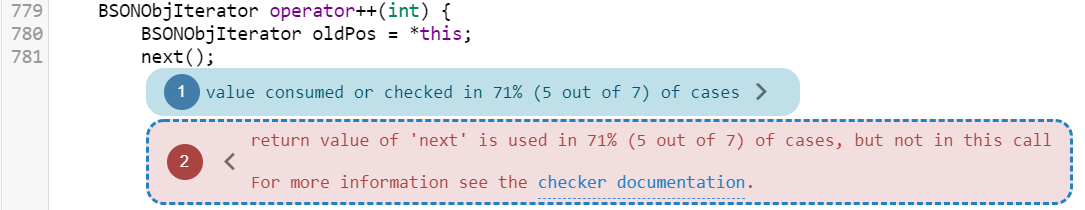
\includegraphics[width=\linewidth]{images/codechecker_first_ss_mongo_single_50.png}
	\caption{A report of the diagnosis of MongoDB's source on CodeChecker with 50\% treshold on a single TU}
\end{figure}

Clang-Tidy is supported by CodeChecker. \cite{codechecker}

\section{Multiple Phase Version}

The updated infrastructure contains two new flags for running Clang-Tidy, multipass-phase and multipass-dir.
Multipass-phase is an enum flag, that has three values, "collect", "compact" and "diagnose" with the latter as default.
Multipass-dir needs a path to a directory where the checkers that support the collect feature can dump their collection datas
that they are going to compact and use later.

\subsection{Collect}

Collect phase, as the name suggest, will have the checkers collect data on each translation unit and write them into unique yaml
files to later reuse this data. This is how you normally run collect phase on the desired files:

\begin{lstlisting}[language={bash}]
	clang-tidy \
	-checks='-*,misc-discarded-return-value' \
	--multipass-phase=collect \
	--multipass-dir='MyCollectionDirectory' \
	-p ./Build \
	a/main.cpp b/main.cpp
\end{lstlisting}

What Discarded Return Value checker (or DRV) does in this phase, is count the amount the declared non-void functions were called,
and count the amount that these function's return values were checked. After finishing counting in one translation unit, it writes the
collected numbers and function names into a yaml file as a struct.  
\par After collecting, you do not get any diagnosis or output text, but the desired amount of (in this case 2) yaml files are going to
be generated.

\begin{lstlisting}[caption={The yaml files containing the collection data},captionpos=b]
bahramib@cc:~/MyFolder/TestFolder/MyCollectionDirectory$ ll
total 8
-rw-r--r-- 1 bahramib bahramib 196 Apr 30 13:00 misc-discarded-return-value.main.cpp.12949585208029997868.yaml
-rw-r--r-- 1 bahramib bahramib 196 Apr 30 13:00 misc-discarded-return-value.main.cpp.4924802982073527590.yaml
\end{lstlisting}

\begin{lstlisting}[caption={Contents of the collection files},captionpos=b]
	# First TU
	---
	- ID:              'c:@S@MyClass@F@check_that#S'
	  Consumed:        3
	  Total:           3
	- ID:              'c:@S@MyClass@F@maybe_check_this#S'
	  Consumed:        0
	  Total:           3
	...
	# Second TU
	---
	- ID:              'c:@S@MyClass@F@check_that#S'
	Consumed:        1
	Total:           3
	- ID:              'c:@S@MyClass@F@maybe_check_this#S'
	Consumed:        3
	Total:           4
	...
\end{lstlisting}

\subsection{Compact}

Compact phase will iterate through the collected data per checker and have the checkers read, use and compact all the data collected
into one yaml file. Flags aside from checks, multipass-phase and multipass-dir have no effect.

\begin{lstlisting}[language={bash}]
	clang-tidy \
	-checks='-*,misc-discarded-return-value' \
	--multipass-phase=compact \
	--multipass-dir='MyCollectionDirectory' \
\end{lstlisting}

DRV reads the data on each function back and constructs new data similar to the previous ones. If one function is called in multiple
translation units, then it simply adds the numbers from the TU's yaml file to the new structure. After it is finished, the data is
written into a single yaml file.
\par This phase does not write anything on standard output either, but will construct the compacted yamls per checker.

\begin{lstlisting}[caption={The new file containing the collected data},captionpos=b]
	bahramib@cc:~/MyFolder/TestFolder/MyCollectionDirectory$ ll
	total 12
	-rw-r--r-- 1 bahramib bahramib 196 Apr 30 13:00 misc-discarded-return-value.main.cpp.12949585208029997868.yaml
	-rw-r--r-- 1 bahramib bahramib 196 Apr 30 13:00 misc-discarded-return-value.main.cpp.4924802982073527590.yaml
	-rw-r--r-- 1 bahramib bahramib 196 Apr 30 13:06 misc-discarded-return-value.yaml
\end{lstlisting}

\begin{lstlisting}[caption={Contents of the compacted file},captionpos=b]
	---
	- ID:              'c:@S@MyClass@F@check_that#S'
	Consumed:        4
	Total:           6
	- ID:              'c:@S@MyClass@F@maybe_check_this#S'
	Consumed:        3
	Total:           7
	...
\end{lstlisting}

\subsection{Diagnose}

For backwards compatibility, the default diagnose phase, will do exactly what the non-multiple
phase Clang-Tidy did, give diagnoses for each translation unit separately, as demonstrated in section \cref{by TU},
if compact has not happened for a checker. Otherwise that checker will read and use the data compacted
in the respective yaml file, and give its diagnosis calculated with project level knowledge.

\begin{lstlisting}[language={bash}]
	clang-tidy \
	-checks='-*,misc-discarded-return-value' \
	--multipass-phase=diagnose \
	--multipass-dir='MyCollectionDirectory' \
	-p ./Build \
	a/main.cpp b/main.cpp
\end{lstlisting}

DRV reads in the compacted data with the call and check amounts for each function and simply desides
if diagnosis is needed or not for each unchecked return value in the current translation unit.
The output is obviously the diagnosis.

\begin{lstlisting}[caption={Diagnosis output with project level knowledge},captionpos=b]
	/home/bahramib/MyFolder/TestFolder/a/main.cpp:12:9: \
	warning: return value of 'check_that' is used \
	in most calls, but noti in this one [misc-discarded-return-value]
	MyClass::check_that();
		^
	/home/bahramib/MyFolder/TestFolder/a/main.cpp:12:9: note: \
	value consumed or checked in 66% (4 out of 6) of cases

	/home/bahramib/MyFolder/TestFolder/a/main.cpp:15:5: \
	warning: return value of 'check_that' is used \
	in most calls, but not in this one [misc-discarded-return-value]
	MyClass::check_that();
	^
	/home/bahramib/MyFolder/TestFolder/a/main.cpp:15:5: note: \
	value consumed or checked in 66% (4 out of 6) of cases
\end{lstlisting}

\begin{figure}
	\label{fig:mongo50multi}
	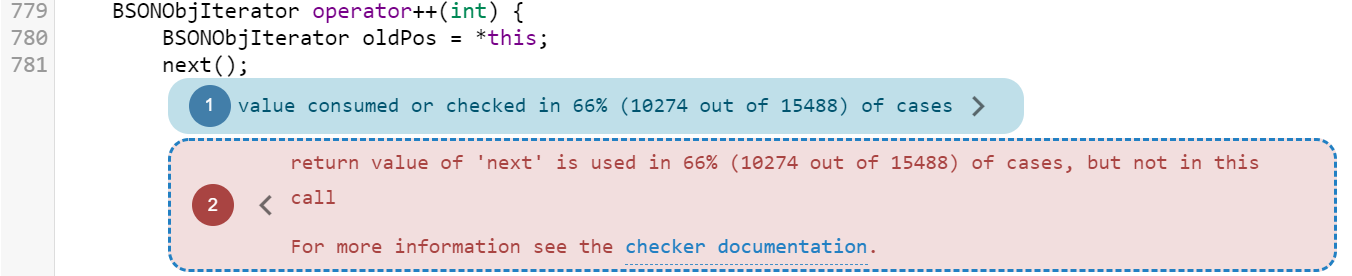
\includegraphics[width=\linewidth]{images/codechecker_first_ss_mongo_multi_50.png}
	\caption{A report of the diagnosis of MongoDB's source on CodeChecker with 50\% treshold and project level knowledge}
\end{figure}

We can clearly conclude, that the multipass diagnosis resulted in different warnings. Figure \cref{fig:mongo50multi}
differs from \cref{fig:mongo50single} in only the percentage, but with a different treshold that could lead to different
results, to either false positives, or hidden true positives. Our own example, however shows both, since we had a call
that used to give warning when diagnosed separately which with project level knowledge does not, and one that did not give
any warnings, but now it gives two, because it passed the treshold.

In \cref{lst:motivation example} we talked about our code getting no warnings without project level knowledge.
After phases collect and compact, however our diagnosis will result in the following:

\begin{lstlisting}
	/home/bahramib/MyFolder/TestFolder/b/vec.cpp:7:15: \
	warning: return value of 'erase' is used \
	in most calls, but not in this one [misc-discarded-return-value]
            c.erase(it);
              ^
/home/bahramib/MyFolder/TestFolder/b/vec.cpp:7:15: note: \
value consumed or checked in 66% (2 out of 3) of cases
\end{lstlisting}

We can clearly see, that our diagnosis gave us the real results this time.
















\iffalse
	\begin{enumerate}
		\item\label{step:first} Donec pretium et quam a cursus. Ut sollicitudin tempus urna et mollis.
		\item Aliquam et aliquam turpis, sed fermentum mauris. Nulla eget ex diam.
		\item Donec eget tellus pharetra, semper neque eget, rutrum diam Step~\ref{step:first}.
	\end{enumerate}

	Praesent porta, metus eget eleifend consequat, eros ligula eleifend ex, a pellentesque mi est vitae urna. Vivamus turpis nunc, iaculis non leo eget, mattis vulputate tellus. Maecenas rutrum eros sem, pharetra interdum nulla porttitor sit amet. In vitae viverra ante. Maecenas sit amet placerat orci, 
	sed tincidunt velit. Vivamus mattis, enim vel suscipit elementum, quam odio venenatis elit\footnote{Phasellus faucibus varius purus, nec tristique enim porta vitae.}, et mollis nulla nunc a risus. Praesent purus magna, tristique sed lacus sit amet, convallis malesuada magna. 

	\begin{description}
		\item[Vestibulum venenatis] malesuada enim, ac auctor erat vestibulum et. Phasellus id purus a leo suscipit accumsan.
		\item[Orci varius natoque] penatibus et magnis dis parturient montes, nascetur ridiculus mus. Nullam interdum rhoncus nisl, vel pharetra arcu euismod sagittis. Vestibulum ac turpis auctor, viverra turpis at, tempus tellus.
		\item[Morbi dignissim] erat ut rutrum aliquet. Nulla eu rutrum urna. Integer non urna at mauris scelerisque rutrum sed non turpis.
	\end{description}

	\subsection{Lists with narrow spacing inbetween items}

	Phasellus ultricies, sapien sit amet ultricies placerat, velit purus viverra ligula, id consequat ipsum odio imperdiet enim:
	\begin{compactenum}
		\item Maecenas eget lobortis leo.
		\item Donec eget libero enim.
		\item In eu eros a eros lacinia maximus ullamcorper eget augue.
	\end{compactenum}

	\bigskip

	In quis turpis metus. Proin maximus nibh et massa eleifend, a feugiat augue porta. Sed eget est purus. Duis in placerat leo. Donec pharetra eros nec enim convallis:
	\begin{compactitem}
		\item Pellentesque odio lacus.
		\item Maximus ut nisl auctor.
		\item Sagittis vulputate lorem.
	\end{compactitem}

	\bigskip

	Vestibulum ante ipsum primis in faucibus orci luctus et ultrices posuere cubilia Curae; Sed lorem libero, dignissim vitae gravida a, ornare vitae est.
	\begin{compactdesc}
		\item[Cras maximus] massa commodo pellentesque viverra.
		\item[Morbi sit] amet ante risus. Aliquam nec sollicitudin mauris
		\item[Ut aliquam rhoncus sapien] luctus viverra arcu iaculis posuere
	\end{compactdesc}


	\section{Images and figures}

	Aliquam vehicula luctus mi a pretium. Nulla quam neque, maximus nec velit in, aliquam mollis tortor. Aliquam erat volutpat. Curabitur vitae laoreet turpis. Integer id diam ligula. Nulla sodales purus id mi consequat, eu venenatis odio pharetra. Cras a arcu quam. Suspendisse augue risus, pulvinar a turpis et, commodo aliquet turpis. Nulla aliquam scelerisque mi eget pharetra. Mauris sed posuere elit, ac lobortis metus. Proin lacinia sit amet diam sed auctor. Nam viverra orci id sapien sollicitudin, a aliquam lacus suscipit, Figure~\ref{fig:example-1}:

	\begin{figure}[H]
		\centering
		
\includegraphics[width=0.6\textwidth,height=100px]{elte_cimer_szines}
		\caption{Quisque ac tincidunt leo}
		\label{fig:example-1}
	\end{figure}

	\subsection{Framing figures}

	Ut aliquet nec neque eget fermentum. Cras volutpat tellus sed placerat elementum. Quisque neque dui, consectetur nec finibus eget, blandit id purus. Nam eget ipsum non nunc placerat interdum.

	\begin{figure}[H]
		\centering
		
\includegraphics[width=0.6\textwidth,height=100px,frame]{elte_cimer_szines}
		\caption{Quisque ac tincidunt leo}
	\end{figure}

	\subsection{Subfigures}

	In non ipsum fermentum urna feugiat rutrum a at odio. Pellentesque habitant morbi tristique senectus et netus et malesuada fames ac turpis egestas. Nulla tincidunt mattis nisl id suscipit. Sed bibendum ac felis sed volutpat. Nam pharetra nisi nec facilisis faucibus. Aenean tristique nec libero non commodo. Nulla egestas laoreet tempus. Nunc eu aliquet nulla, quis vehicula dui. Proin ac risus sodales, gravida nisi vitae, efficitur neque, Figure~\ref{fig:example-2}:

	\begin{figure}[H]
		\centering
		\subcaptionbox{Vestibulum quis mattis urna}{
			
\includegraphics[width=0.45\linewidth]{elte_cimer_szines}}
		\hspace{5pt}
		\subcaptionbox{Donec hendrerit quis dui sit amet venenatis}{
			
\includegraphics[width=0.45\linewidth]{elte_cimer_szines}}
		\caption{Aenean porttitor mi volutpat massa gravida}
		\label{fig:example-2}
	\end{figure}

	Nam et nunc eget elit tincidunt sollicitudin. Quisque ligula ipsum, tempor vitae tortor ut, commodo rhoncus diam. Pellentesque habitant morbi tristique senectus et netus et malesuada fames ac turpis egestas. Phasellus vehicula quam dui, eu convallis metus porta ac.


	\section{Tables}

	Nam magna ex, euismod nec interdum sed, sagittis nec leo. Nam blandit massa bibendum mattis tristique. Phasellus tortor ligula, sodales a consectetur vitae, placerat vitae dolor. Aenean consequat in quam ac mollis. 

	\begin{table}[H]
		\centering
		\begin{tabular}{ | m{0.25\textwidth} | m{0.65\textwidth} | }
			\hline
			\textbf{Phasellus tortor} & \textbf{Aenean consequat} \\
			\hline \hline
			\emph{Sed malesuada} & Aliquam aliquam velit in convallis ultrices. \\
			\hline
			\emph{Purus sagittis} &  Quisque lobortis eros vitae urna lacinia euismod. \\
			\hline
			\emph{Pellentesque} & Curabitur ac lacus pellentesque, eleifend sem ut, placerat enim. Ut auctor tempor odio ut dapibus. \\
			\hline
		\end{tabular}
		\caption{Maecenas tincidunt non justo quis accumsan}
		\label{tab:example-1}
	\end{table}

	\subsection{Multi rows and multi columns}

	Mauris a dapibus lectus. Vestibulum commodo nibh ante, ut maximus magna eleifend vel. Integer vehicula elit non lacus lacinia, vitae porttitor dolor ultrices. Vivamus gravida faucibus efficitur. Ut non erat quis arcu vehicula lacinia. Nulla felis mauris, laoreet sed malesuada in, euismod et lacus. Aenean at finibus ipsum. Pellentesque dignissim elit sit amet lacus congue vulputate.

	\begin{table}[htb]
		\centering
		\begin{tabular}{ | c | r | r | r | r | r | r | }
			\hline
			\multirow{2}{*}{\textbf{Quisque}} & \multicolumn{2}{ c | }{\textbf{Suspendisse}} & \multicolumn{2}{ c | }{\textbf{Aliquam}} & \multicolumn{2}{ c | }{\textbf{Vivamus}} \\
			\cline{2-7}
			& Proin & Nunc & Proin & Nunc & Proin & Nunc \\
			\hline \hline		
			Leo & 2,80 MB & 100\% & 232 KB & 8,09\% & 248 KB & 8,64\% \\
			\hline
			Vel & 9,60 MB & 100\% & 564 KB & 5,74\% & 292 KB & 2,97\% \\
			\hline
			Auge & 78,2 MB & 100\% & 52,3 MB & 66,88\% & 3,22 MB & 4,12\% \\
			\hline 
		\end{tabular}
		\caption[Rövid cím a táblázatjegyzékbe]{Vivamus ac arcu fringilla, fermentum neque sed, interdum erat. Mauris bibendum mauris vitae enim mollis, et eleifend turpis aliquet.}
		\label{tab:example-2}
	\end{table}

	\subsection{Long tables over multiple pages}

	Nunc porta placerat leo, sit amet porttitor dui porta molestie. Aliquam at fermentum mi. Maecenas vitae lorem at leo tincidunt volutpat at nec tortor. Vivamus semper lacus eu diam laoreet congue. Vivamus in ipsum risus. Nulla ullamcorper finibus mauris non aliquet. Vivamus elementum rhoncus ex ut porttitor.

	\begin{center}
		\begin{longtable}{ | p{0.3\textwidth} | p{0.7\textwidth} | }
			
			\hline
			\multicolumn{2}{|c|}{\textbf{Praesent aliquam mauris enim}}
			\\ \hline
			
			\emph{Suspendisse potenti} & \emph{Lorem ipsum dolor sit amet}
			\\ \hline \hline
			\endfirsthead % table header on first page
			
			\hline
			\emph{Suspendisse potenti} & \emph{Lorem ipsum dolor sit amet}
			\\ \hline \hline
			\endhead % table header on further pages
			
			\hline
			\endfoot % table footer on previous pages
			
			\endlastfoot % table footer on last page
			
			\emph{Praesent}
			& Nulla ultrices et libero sit amet fringilla. Nunc scelerisque ante tempus sapien placerat convallis.
			\\ \hline
			
			\emph{Luctus}
			& Integer hendrerit erat massa, non hendrerit risus convallis at. Curabitur ultrices, justo in imperdiet condimentum, neque tortor luctus enim, luctus posuere massa erat vitae nibh.
			\\ \hline
			
			\emph{Egestas}
			& Duis fermentum feugiat augue in blandit. Mauris a tempor felis. Pellentesque ultricies tristique dignissim. Pellentesque aliquam semper tristique. Nam nec egestas dolor. Vestibulum id elit quis enim fringilla tempor eu a mauris. Aliquam vitae lacus tellus. Phasellus mauris lectus, aliquam id leo eget, auctor dapibus magna. Fusce lacinia felis ac elit luctus luctus.
			\\ \hline
			
			\emph{Dignissim}
			& Praesent aliquam mauris enim, vestibulum posuere massa facilisis in. Suspendisse potenti. Nam quam purus, rutrum eu augue ut, varius vehicula tellus. Fusce dui diam, aliquet sit amet eros at, sollicitudin facilisis quam. Phasellus tempor metus vel augue gravida pretium. Proin aliquam aliquam blandit. Nulla id tempus mi. Fusce in aliquam tortor.
			\\ \hline
			
			\emph{Pellentesque}
			& Donec felis nibh, imperdiet a arcu non, vehicula gravida nibh. Quisque interdum sapien eu massa commodo, ac elementum felis faucibus.
			\\ \hline
			
			\emph{Molestie}
			& Cras ullamcorper tellus et auctor ultricies. Maecenas tincidunt euismod lectus nec venenatis. Suspendisse potenti. Pellentesque pretium nunc ut euismod cursus. Nam venenatis condimentum quam. Curabitur suscipit efficitur aliquet. Interdum et malesuada fames ac ante ipsum primis in faucibus.
			\\ \hline
			
			\emph{Vivamus semper}
			& In purus purus, faucibus eu libero vulputate, tristique sodales nunc. Nulla ut gravida dolor. Fusce vel pellentesque mi, vel efficitur eros. Nunc vitae elit tellus. Sed vestibulum auctor consequat. 
			\\ \hline
			
			\emph{Condimentum}
			& Nulla scelerisque, leo et facilisis pretium, risus enim cursus turpis, eu suscipit ipsum ipsum in mauris. Praesent eget pulvinar ipsum, suscipit interdum nunc. Nam varius massa ut justo ullamcorper sollicitudin. Vivamus facilisis suscipit neque, eu fermentum risus. Ut at mi mauris.
			\\ \hline
			
			\caption{Praesent ullamcorper consequat tellus ut eleifend}
			\label{tab:example-3}		
		\end{longtable}
	\end{center}
\fi